
Let us start from the 2D steady state heat diffusion equation:
\begin{equation}
    \vec{\nabla} \cdot k \vec{\nabla} T + H=0
\end{equation}
Just as in the 1D case this equation can be split in two separate first order differential equations:
\begin{equation}
    \underbrace{-\vec{\nabla}\cdot \vec{q} + H=0}_{\text{ODE 1}} \quad ; \quad \underbrace{\vec{q}=-k\vec{\nabla } T}_{\text{ODE 2}}
\end{equation}
Let $N^\uptheta_i$ be the temperature basis functions so that the temperature inside an element is given by
\begin{equation}
T_h (\vec{r}) = \sum_{i=1}^m N_i^\uptheta (\vec{r}) \; T_i = \vec{N^\uptheta}\cdot \vec{T}
\end{equation}
where $\vec{T}$ is a vector of length $m$, the number of nodes per element. Similarly we let the basis function for the heat flux be
\begin{equation}
\qhx(x,y) = \sum_{i=1}^m N_i^q (x,y) \qix = \vec{N^q}\cdot \vec{\qx}
\end{equation}
\begin{equation}
\qhy(x,y) = \sum_{i=1}^m N_i^q (x,y) \qiy = \vec{N^q}\cdot \vec{\qy}
\end{equation}
where $\vec{\qx}$, $\vec{\qy}$ and $\vec{N}^q$ 
are vectors of length $m$ too. Implicitly if $m$ is the same for temperature and heat flux, then $N^\uptheta = N^q$.

Let us establish the weak forms of the 1st order ODEs. 


\paragraph{ODE 1} This results in:
\begin{eqnarray}
\int_\Omega {N^\uptheta_i} \vec{\nabla} \cdot \vec{q} \; dV = \int_\Omega {N^\uptheta_i} H \; dV
\label{eq:SSD2D}
\end{eqnarray}
Using the product rule which states:
\[
\vec{\nabla} \cdot ({N^\uptheta_i}\vec{q})={N^\uptheta_i}\vec{\nabla} \cdot \vec{q} 
+ \vec{\nabla}{N^\uptheta_i} \cdot \vec{q} 
\qquad
\Rightarrow
\qquad
{N^\uptheta_i}\vec{\nabla} \cdot \vec{q}=\vec{\nabla} \cdot ({N^\uptheta_i}\vec{q})- 
\vec{\nabla}{N^\uptheta_i} \cdot \vec{q}
\]
which we insert in Eq.~(\ref{eq:SSD2D}) results in 
\begin{equation}
\int_{\Omega} \vec{\nabla} \cdot ({N^\uptheta_i} \vec{q}) dV - 
\int_{\Omega} \vec{\nabla} {N^\uptheta_i} \cdot \vec{q} dV = \int_{\Omega} {N^\uptheta_i} H dV
\label{eq:SSD2D1}
\end{equation}
Using the divergence theorem 
$\int_\Omega \vec{\nabla} \cdot \vec{F} \; d\Omega = \int_{d\Omega}(\vec{F} \cdot \vec{n}) \; dS$ 
 applied to Eq.~(\ref{eq:SSD2D1}) leads to
\begin{equation}
\int_{d\Omega}{N^\uptheta_i} \vec{\hat{q}} \cdot \vec{n} \; dS  - 
\int_{\Omega} \vec{\nabla} {N^\uptheta_i} \cdot \vec{q} \; dV = 
\int_{\Omega} {N^\uptheta_i} H  \; dV
\end{equation}

Here $\vec{n}$ is the outward vector everywhere on the boundary. 
The exact solution $\vec{q}=(\qx,\qy)$ can be approximated with $\vec{q}_h$ in a  finite element space, same for the approximation of the flux at the boundary $\hat{q}=\hat{q_h}$ which takes a special form in the context of the DG methods (as reflected by the presence of the hat).
\begin{equation}
\underbrace{ \int_{d\Omega}{N^\uptheta_i} \vec{\hat{q_h}} \cdot \vec{n} \; dS}_{A } - 
\underbrace{ \int_{\Omega} \vec{\nabla} {N^\uptheta_i} \cdot \vec{q_h} \; dV}_{B} = 
\underbrace{\int_{\Omega} {N^\uptheta_i} H  \;dV }_C
\label{eq:q2dss}
\end{equation}
%To make things very explicit, we can split the heat flux in its $x$ and $y$ component in the above equation:
%\begin{equation}
%\int_{d\Omega}  {N^\theta} (\hat{\qx} \nx + \hat{\qy} \ny) \; dS  -  
%\int_{\Omega} ( \partial_x N^\theta \qx   + 
%\partial_y N^\theta \qy ) \; dV = 
%\int_{\Omega} {N^\theta} H dV
%\label{eq:q2dss}
%\end{equation}
The middle and right terms are explained in Section~\ref{ss:hte_diff}, 
so we will focus on the left term only (i.e. the one with the fluxes).
In all what follows blue symbols belong the the element under consideration 
and brown symbols belong to its neighbour(s).

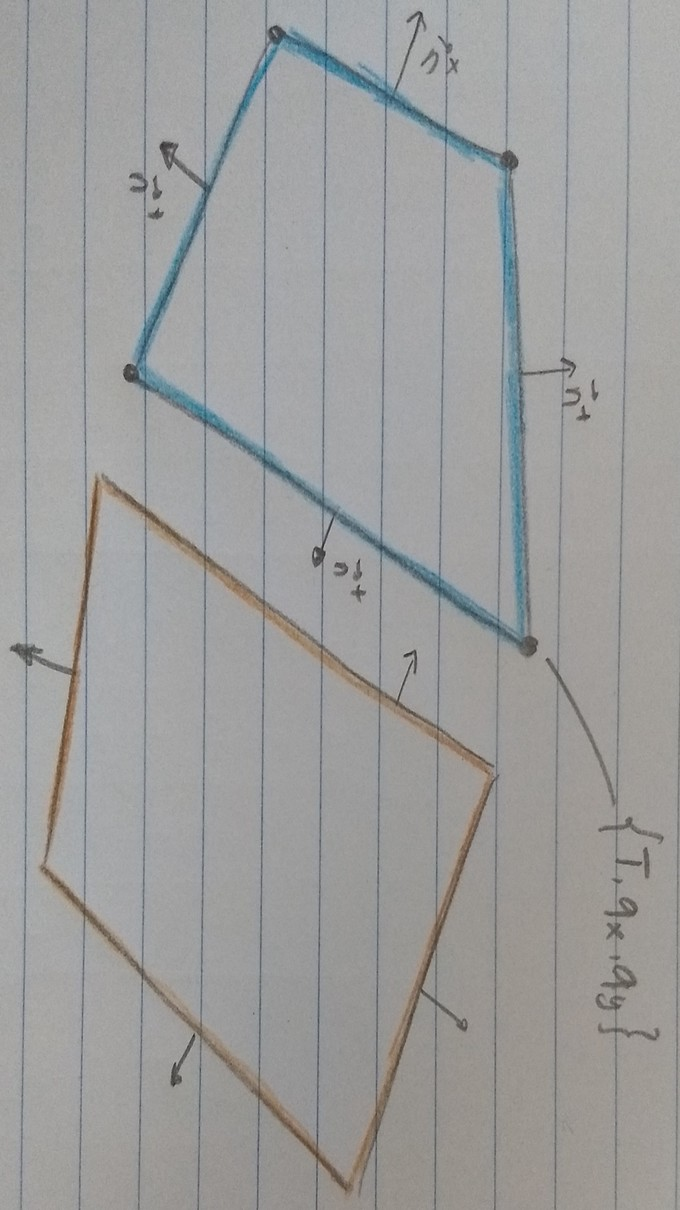
\includegraphics[width=5cm,angle=90]{images/dgfem/elts}
%Here the blue color (before: $el$ superscript) indicates that it belongs to the element of interest and brown color (before: the $nb$ superscript) 
%denotes the values belonging to the neighbouring element. 
$\vec{n}^+$ indicates the outward vector at the boundary and $\vec{n}^-$ is 
the outward vector of the neighbouring element.

Let us turn to the book for useful definitions:
\begin{itemize}
\item
\underline{Definition of jump operators} The square brackets denote the jump operator:
\begin{eqnarray}
[\vec{q}_h] &=& \vec{\color{blue}q}_h \cdot \vec{n}^+ 
+ \vec{\color{brown} q}_h \cdot \vec{n}^- 
\qquad \text{or} \qquad 
[\vec{q}_h]= (\vec{\color{blue}q}_h - \vec{\color{brown}q}_h) \cdot \vec{n}^+    \nn\\
\left[T_h\right] &=& \blueT_h \vec{n}^+ + {\brownT}_h \vec{n}^-  \qquad \text{or} \qquad 
[T_h]=(\blueT_h  - \brownT_h ) \; \vec{n}^+ 
\end{eqnarray}
%[q_{h,x}]=q_{h,x}^{el}n_x^+ + q_{h,x}^{nb}n_x^- \nn \\
%[q_{h,y}]=q_{h,y}^{el}n_y^+ + q_{h,y}^{nb}n_y^- \nn \\

Note that $[\vec{q}_h]$ is a scalar function which involves the
normal components only; while $[T_h]$ is a vector function. 

\item
\underline{Definition of average operators} The curly brackets indicate the average operator
\begin{eqnarray}
\{ \vec{q}_h \}&=&\frac{1}{2}(\vec{\color{blue}q}_h + \vec{\color{brown}q}_h)
\qquad \text{so} \quad 
\{\qhx\}=\frac{1}{2}(\blueqx_h + \brownqx_h) 
\qquad \text{and}
\qquad  \{\qhy\}=\frac{1}{2}(\blueqy_h + \brownqy_h) \nn \\
\{T_h\}&=&\frac{1}{2}(\blueT_h + \brownT_h) \nn 
\end{eqnarray}
Note that $\{ \vec{q}_h \}$ is a vector, while 
$\{T_h\}$ is a scalar.

\item
\underline{Definitions of fluxes} In the LDG method the boundary flux $\vec{\hat{q}}$ is defined as 
\[
\vec{\hat{q_h}} = \{ \vec{q_h} \} -{\cal{E}} [T_h]- \vec{\cal{C}}  [\vec{q_h}] 
\]
where ${\cal{E}}$ is a scalar (since $[T_h]$ is a vector)
and $\vec{\cal C}$ is a vector (since $[\vec{q}_h]$ is a scalar).
To be once again very explicit:
\begin{eqnarray}
\hat{\qhx} 
&=& \{\qhx\} -{\cal{E}} [T_h]_x- {\cal{C}}_x  [\vec{q}_h] \nn\\
&=& \frac{1}{2}(\blueqx_h + \brownqx_h)
-{\cal{E}} (\blueT_h {n}_x^+ + \brownT_h {n}_x^-)
-{\cal{C}}_x  
(\vec{\color{blue}q}_h \cdot \vec{n}^+ +\vec{\color{brown}q}_h \cdot \vec{n}^-) \label{flux2Da}\\
\hat{\qhy} 
&=& \{\qhy\} -{\cal{E}} [T_h]_y- {\cal{C}}_y  [\vec{q}_h] \nn\\
&=& \frac{1}{2}(\blueqy_h + \brownqy_h)  
-{\cal{E}}  (\blueT_h {n}_y^+ + \brownT_h {n}_y^-)
-{\cal{C}}_y  (\vec{\color{blue} q}_h \cdot \vec{n}^+ +\vec{\color{brown}q}_h \cdot \vec{n}^-) \label{flux2Db}
\end{eqnarray}

\begin{remark}
Note that in the the book the note under table 4.1 states that the $C_{ij}$ 
coefficients are constant matrices, which is quite misleading since some are actually scalars and others vectors.
\end{remark}

\end{itemize}


Filling Eqs.~(\ref{flux2Da},\ref{flux2Db}) into Eq.~(\ref{eq:q2dss}) leads to
%(note that I have introduced the upperscript + on the normal components 
%because the integration is on the boundary of the element - does that make sense?)


\begin{eqnarray}
A&=& \int_{\partial\Omega} N^\uptheta_i \vec{\hat{q_h}} \cdot \vec{n} \; dS \nn\\ 
&=&
\int_{\partial\Omega} N^\uptheta_i \left[ \{ \vec{q_h} \} -{\cal{E}} [T_h]- \vec{\cal{C}}  [\vec{q_h}] \right] \cdot \vec{n}^+ \; dS  \nn\\
&=&
\int_{\partial\Omega}{N^\uptheta_i} \left[ \frac{1}{2}(\vec{\color{blue}q}_h + \vec{\color{brown}q}_h) 
-{\cal{E}} (\blueT_h \vec{n}^+ + \brownT_h \vec{n}^-)- \vec{\cal{C}}  [\vec{q_h}] \right] \cdot \vec{n}^+ \; dS  \nn\\
&=&
\int_{\partial\Omega}{N^\uptheta_i} \left[ \frac{1}{2}(\vec{\color{blue}q}_h + \vec{\color{brown}q}_h)\cdot\vec{n}^+ 
  -{\cal{E}} (\blueT_h \vec{n}^+ + \brownT_h \vec{n}^-) \cdot \vec{n}^+
- \vec{\cal{C}} \cdot \vec{n}^+ [\vec{q_h}] \right] \; dS  \nn\\
&=&
\int_{\partial\Omega}{N^\uptheta_i} \left[ \frac{1}{2}(\vec{\color{blue}q}_h + \vec{\color{brown}q}_h)\cdot\vec{n}^+  -{\cal{E}} (\blueT_h -\brownT_h ) 
- (\vec{\cal{C}} \cdot \vec{n}^+) 
(\vec{\color{blue}q}_h - \vec{\color{brown}q}_h) \cdot \vec{n}^+
\right] \; dS  \qquad \text{since} \quad  \vec{n}^+\!\cdot\!\vec{n}^+ =1 \quad  \vec{n}^+\!\cdot\!\vec{n}^- =-1 \nn\\
&=&
\int_{\partial\Omega}{N^\uptheta_i} \left[
\left(\frac{1}{2} - \vec{\cal{C}} \cdot \vec{n}^+ \right) \vec{\color{blue}q}_h\cdot\vec{n}^+
- {\cal{E}} \blueT_h
\right] \; dS 
+ 
\int_{\partial\Omega}{N^\uptheta_i} \left[
\left(\frac{1}{2} + \vec{\cal{C}} \cdot \vec{n}^+ \right)
\vec{\color{brown}q}_h \cdot\vec{n}^+
+ {\cal{E}} \brownT_h
\right] \; dS  \nn \\
&=&
\int_{\partial\Omega}{N^\uptheta_i} 
\left(\frac{1}{2} - \vec{\cal{C}} \cdot \vec{n}^+ \right) \vec{\color{blue}q}_h\cdot\vec{n}^+ \; dS 
- \int_{\partial\Omega}{N^\uptheta_i}  {\cal{E}} \blueT_h  \; dS 
+ 
\int_{\partial\Omega}{N^\uptheta_i} \left(\frac{1}{2} + \vec{\cal{C}} \cdot \vec{n}^+ \right)
\vec{\color{brown}q}_h \cdot\vec{n}^+   \; dS
+
\int_{\partial\Omega}{N^\uptheta_i}   {\cal{E}} \brownT_h   \; dS  \nn \\
&=& A_1 + A_2 + A_3 + A_4 
\end{eqnarray}
In order to simplify notations we choose $N^q=N^\uptheta=N$ and drop the $h$ subscripts.

\begin{eqnarray}
A_1 
&=& \int_{\partial\Omega}{N_i} \left(\frac{1}{2} - \vec{\cal{C}} \cdot \vec{n}^+ \right) \vec{\color{blue}q}\cdot\vec{n}^+ \; dS \nn \\
&=& \int_{\partial\Omega}{N_i} \left(\frac{1}{2} - \vec{\cal{C}} \cdot \vec{n}^+ \right) ({\color{blue}q}_x n^+_x  +   {\color{blue}q}_y {n}_y^+) \; dS \nn \\
&=& \int_{\partial\Omega}{N_i} \left(\frac{1}{2} - \vec{\cal{C}} \cdot \vec{n}^+ \right) {\color{blue}q}_x n^+_x   \; dS 
+ \int_{\partial\Omega}{N_i} \left(\frac{1}{2} - \vec{\cal{C}} \cdot \vec{n}^+ \right)  {\color{blue}q}_y {n}_y^+ \; dS \nn \\
\Rightarrow {\vec A}_1
&=& \left( \int_{\partial\Omega}  \left(\frac{1}{2} - \vec{\cal{C}} \cdot \vec{n}^+ \right) \vec{N}^T \vec{N} n^+_x  \; dS  \right) \cdot {\color{blue}\vec{\qx}}  
+ \left( \int_{\partial\Omega}  \left(\frac{1}{2} - \vec{\cal{C}} \cdot \vec{n}^+ \right) \vec{N}^T \vec{N} n^+_y  \; dS  \right) \cdot {\color{blue}\vec{\qy}}  \\
A_2 &=& - \int_{\partial\Omega}{N_i}  {\cal{E}} \blueT  \; dS \nn\\
\Rightarrow {\vec A}_2 &=& - \left( \int_{\partial\Omega}   {\cal{E}}   \vec{N}^T \vec{N} dS \right) \cdot \vec{\blueT} \\
A_3 
&=& \int_{\partial\Omega}{N^\uptheta_i} \left(\frac{1}{2} + \vec{\cal{C}} \cdot \vec{n}^+ \right)
 \vec{\color{brown}q} \cdot\vec{n}^+   \; dS \nn\\
&=& \int_{\partial\Omega}{N^\uptheta_i} \left(\frac{1}{2} + \vec{\cal{C}} \cdot \vec{n}^+ \right)
 ({\color{brown}q}_x {n}_x^+  +  {\color{brown}q}_y {n}_y^+       )  \; dS \nn\\
&=& 
\int_{\partial\Omega}{N^\uptheta_i} \left(\frac{1}{2} + \vec{\cal{C}} \cdot \vec{n}^+ \right)  {\color{brown}q}_x {n}_x^+    \; dS 
+ \int_{\partial\Omega}{N^\uptheta_i} \left(\frac{1}{2} + \vec{\cal{C}} \cdot \vec{n}^+ \right)   {\color{brown}q}_y {n}_y^+    \; dS \nn\\
\Rightarrow {\vec A}_3 &=&
  \left(\int_{\partial\Omega} \left(\frac{1}{2} + \vec{\cal{C}} \cdot \vec{n}^+ \right) \vec{N}^T \vec{N} {n}_x^+    \; dS \right) \cdot  {\color{brown}\vec{\qx}}
+ \left(\int_{\partial\Omega} \left(\frac{1}{2} + \vec{\cal{C}} \cdot \vec{n}^+ \right) \vec{N}^T \vec{N} {n}_y^+    \; dS \right) \cdot  {\color{brown}\vec{\qy}} \\
A_4 &=& \int_{\partial\Omega}{N_i}   {\cal{E}}  \brownT   \; dS  \nn\\
\Rightarrow {\vec A}_4 &=&  \left( \int_{\partial\Omega}   {\cal{E}}   \vec{N}^T \vec{N} dS \right) \cdot \vec{\brownT} \\ 
B 
&=& \int_{\Omega} \vec{\nabla} {N_i} \cdot \vec{\color{blue} q} \; dV  \nn \\
&=& \int_{\Omega} (\partial_x N_i {\color{blue}q}_x + \partial_y N_i {\color{blue}q}_y )   \; dV  \nn \\
&=& \int_{\Omega} \partial_x N_i {\color{blue}q}_x   \; dV   
 +  \int_{\Omega} \partial_y N_i {\color{blue}q}_y   \; dV  \nn \\
\Rightarrow {\vec B} &=& 
  \left(\int_{\Omega} \partial_x \vec{N}^T \vec{N}   \; dV \right)\cdot {\color{blue}\vec{\qx}}  
+ \left(\int_{\Omega} \partial_y \vec{N}^T \vec{N}   \; dV \right)\cdot {\color{blue}\vec{\qy}}  \\
C &=& \int_{\Omega} {N_i} H  \;dV \nn \\
\Rightarrow {\vec C} &=& \int_{\Omega} \vec{N}^T H  \;dV  
\end{eqnarray}


The expressions above find their equivalent in the book (NB stands for neighbour):
\begin{center}
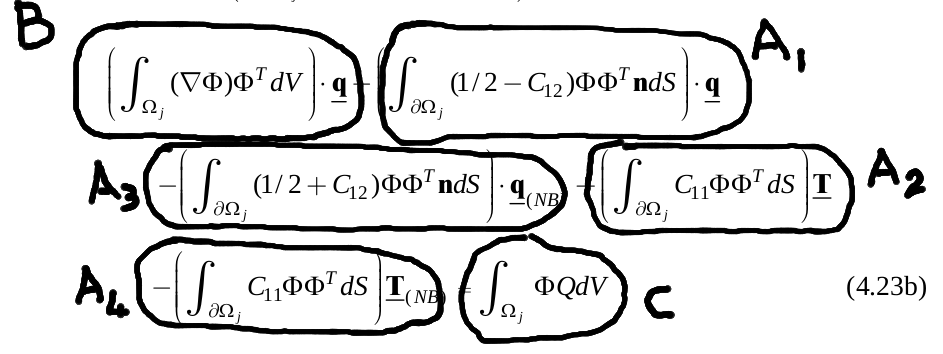
\includegraphics[width=11cm]{images/dgfem/li_01}\\
{\captionfont Note that in the book we have: $C_{12}={\bm C}_{12}\cdot {\bm n}^+ \rightarrow \vec{\cal C}\cdot\vec{n}^+$;
$C_{11} \rightarrow {\cal E}$}
\end{center}






%---------------------------------------------------
\paragraph{ODE 2} The weak form of Ode \#2 writes:

\[
\int_\Omega N_i^q (\vec{q} + k\vec{\nabla } T ) dV = 0
\]
or, (once again we drop the superscript on the shape functions and the $h$):
\[
\int_\Omega N_i \vec{q} \;  dV + \int_\Omega N_i k\vec{\nabla } T \; dV = 0
\]
We then use $\int_\Omega \vec\nabla f \; dV = \int_{\partial\Omega} f \vec{dS}$
and as before the temperature on the edge integral should be $\hat{T}$:
\[
\int_\Omega N_i \vec{q} \;  dV + \int_{\partial\Omega}  k N_i \hat{T} \; \vec{n}^+  dS - \int_\Omega \vec\nabla (k N_i)   T \; dV = 0
\]


or, if decomposed in a 2D Cartesian axis system 
\begin{eqnarray}
0
%&=&\int_\Omega N_i \left( \qx + k  \frac{\partial T}{\partial x} \right) \; dV \nn\\
%&=&\int_\Omega N_i  \qx^h dV
%+ \int_\Omega N_i k  \frac{\partial T^h}{\partial x}  \; d\Omega \nn\\
&=&\int_\Omega N_i  \qx dV 
+\int_{\partial\Omega} N_i k \hat{T} \; n^+_x dS
-\int_\Omega \partial_x ( k N_i) \;  T \; dV \nn\\
0
%&=&\int_\Omega N_i \left( \qy^h + k  \frac{\partial T^h}{\partial y} \right) \; dV \nn\\
%&=&\int_\Omega N_i  \qy^h dV
%+ \int_\Omega N_i k  \frac{\partial T^h}{\partial y}  \; d\Omega \nn\\
&=&\int_\Omega N_i  \qy^h dV 
+\int_{\partial\Omega} N_i k \hat{T} \; n^+_y dS
-\int_\Omega \partial_y (k N_i) \;  T \; dV \nn
\end{eqnarray}
%Both can be summed together and creating the vector $\vec{N}=(N_i,N_i)= N_i(\vec{e}_x+\vec{e}_y)$ then we get 
%\[
%\int_\Omega \vec{N}_i \cdot \vec{q}^h dV 
%+\int_{\partial\Omega} k \hat{T} \vec{N}\cdot \vec{n}^+  dS
%-\int_\Omega \vec{\nabla}\cdot (\vec{N}_i k) \;  T \; dV 
%=0
%\]
which (aside from a minus sign coming from a different definition of the heat flux) is 'identical' to the book
(although the notations in the book are hella confusing):
\begin{center}
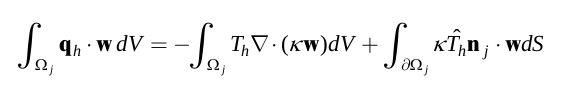
\includegraphics[width=8cm]{images/dgfem/li_02} (with $\kappa \rightarrow k$, ${\bm w}\rightarrow \vec{N}$)
\end{center}


\begin{eqnarray}
D &=&  \\
E &=&  \\
F &=&  \\
G &=&  \\
H &=&  \\
I &=&  \\
\end{eqnarray}
























\par\noindent\rule{\textwidth}{0.4pt}


We start from the steady state (no advection) energy equation:
\[
\vec\nabla\cdot (k \vec\nabla T) + Q = 0
\]
where $Q$ is a source term.
As we did in 1D we tranform this equation by reintroducing the heat flux
\footnote{\url{https://en.wikipedia.org/wiki/Thermal_conduction}} $\vec{q}$ 
\begin{eqnarray}
\vec q &=& - k \vec\nabla T \\
\vec\nabla \cdot \vec q &=& Q
\end{eqnarray}
We then multiply these two equations with the test functions $\vec{N}_q$ (this one 
is vector valued) and 
$N_T$ respectively and integrate over the element $e$ under consideration:
\begin{eqnarray}
\int_{\Omega_e} \vec{N}_q \cdot  \vec q  \; dV &=& - \int_{\Omega_e} \vec{N}_q \cdot k \vec\nabla T\; dV \\
\int_{\Omega_e} N_T \vec\nabla \cdot \vec q \;  dV &=& \int_{\Omega_e} N_T Q \; dV
\end{eqnarray}
We then use integration by parts to make fluxes appear (and assume $k$ is constant within 
the element). We have
\begin{eqnarray}
\int_{\Omega_e} \vec{N}_q \cdot k \vec\nabla T \; dV 
&=& \int_{\Gamma_e} kT \;  \vec{N}_q \cdot \vec{n} \; dS 
- \int _{\Omega_e}  kT \;  \vec\nabla\cdot \vec{N}_q  \;  dV \\
\int_{\Omega_e} N_T \vec\nabla \cdot \vec q \; dV 
&=& \int_{\Gamma_e} {N}_T \vec{q} \cdot \vec{n}  \; dS
- \int_{\Omega_e} \vec\nabla N_T \cdot \vec q \; dV 
\end{eqnarray}
We then finally obtain the weak forms that are to be discretised:
\begin{eqnarray}
\int_{\Omega_e} \vec{N}_q \cdot  \vec q \; dV &=& 
-\int_{\Gamma_e} kT \;  \vec{N}_q \cdot \vec{n} \; dS 
+ \int _{\Omega_e}  kT \;  \vec\nabla\cdot \vec{N}_q  \;  dV \\
\int_{\Gamma_e}    {N}_T  \vec{q}\cdot \vec{n}  \; dS
- \int_{\Omega_e} \vec\nabla N_T \cdot \vec q \; dV 
&=& \int_{\Omega_e} N_T Q \; dV
\end{eqnarray}

We seek to approximate the exact solution $(\vec{q},T)$ with functions $(\vec{q}_h,T_h)$ inside the element so we 
now have 
\begin{eqnarray}
\int_{\Omega_e} \vec{N}_q \cdot  \vec q_h \; dV &=& 
-\int_{\Gamma_e} k \hat{T}_h \;  \vec{N}_q \cdot \vec{n} \; dS 
+ \int _{\Omega_e}  k T_h \;  \vec\nabla\cdot \vec{N}_q  \;  dV \\
\int_{\Gamma_e}    {N}_T \hat{\vec{q}}_h \cdot \vec{n}  \; dS
- \int_{\Omega_e} \vec\nabla N_T \cdot \vec{q}_h \; dV 
&=& \int_{\Omega_e} N_T Q \; dV
\end{eqnarray}
where the numerical fluxes are the approximations to $(\vec{q},T)$ on the boundary of element $e$.
As before we must now specify these fluxes inside the domain and also on the boundaries. These
can obviously not be chosen at will since they must at least render the discontinuous formulation stable.



The following table is taken from Li \cite{li06} and lists the numerical fluxes 
that are considered consistent and stable for the solution of the steady state heat conduction 
problems \cite{arbc02,cacp00}:
\begin{center}
\begin{tabular}{lll}
\hline
Method & $\hat{\vec{q}}_h$ & $\hat{T}_h$ \\
\hline
LDG \cite{cosh98} & $\{ \vec{q}_h \}$  & \\
DG  \cite{cacp00} & \\
Brezzi et al (2000) \cite{brmm00} &\\
IP \cite{dodu76} & \\
Bassi-Rebay \cite{barm97} &\\
NIPG \cite{riwg99} & \\
\hline
\end{tabular}
\end{center}
where the $C$ coefficients are matrices ?!



\index{general}{Average Operator}
\index{general}{Jump Operator}
The average operator and jump operators in the table are defined as follows:
let $\Gamma_{12}$ be an interior edge shared by elements $1$ and $2$ and let us 
define the unit normal vectors $\vec{n}_1$ and $\vec{n}_2$ on $\Gamma_{12}$ 
pointing exterior to element 1 and 2, respectively.



\end{document}

